\documentclass[10pt,aspectratio=169]{beamer}

%================================================
% Theme
%================================================
\usetheme[numbering=fraction,progressbar=frametitle]{metropolis}

%================================================
% Packages
%================================================
\usepackage{amsmath,amssymb}
\usepackage{booktabs}
\usepackage{array}
\usepackage{tikz}
\usetikzlibrary{automata,positioning,arrows.meta,calc}
\usepackage{xcolor}
\usepackage{listings}

%================================================
% Metadata
%================================================
\newcommand{\LastCompiled}{\today}

\title{Theory of Computation}
\subtitle{Lecture 3: Deterministic Finite Automata}
\author{Sheikh Azizul Hakim\\Lecturer, Department of CSE, BUET}
\date{Last compiled: \LastCompiled}

%================================================
% Convenience Macros
%================================================
\newcommand{\eps}{\varepsilon}
\newcommand{\blank}{\sqcup}
\newcommand{\Yes}{\textsc{Yes}}
\newcommand{\No}{\textsc{No}}
\newcommand{\lang}[1]{\mathsf{#1}}
\newcommand{\dfa}{M=(Q,\Sigma,\delta,q_0,F)}

\tikzset{
  dfastate/.style={state,minimum size=8mm,inner sep=1pt},
  smallstate/.style={state,minimum size=7mm,inner sep=1pt},
  every edge/.style={draw,->,>=Stealth,shorten >=1pt},
}

%================================================
% Listings
%================================================
\lstdefinestyle{code}{
  basicstyle=\ttfamily\small,
  frame=single,
  backgroundcolor=\color{black!4},
  rulecolor=\color{black!20},
  showstringspaces=false,
  columns=fullflexible,
  keepspaces=true
}
\lstset{style=code}

%================================================
\begin{document}

%================================================
\maketitle

%================================================
\begin{frame}[standout]
How do we describe finite memory precisely?
\end{frame}

%================================================
\section{3A. The Concept of State \& Mathematical Models}

%================================================
\begin{frame}{Where We Are in the Story}

\begin{center}
\begin{tabular}{lll}
\toprule
\textbf{Lecture} & \textbf{Question} & \textbf{Main idea}\\
\midrule
1 & Why study computation? & Limits of machines\\
2 & What are problems? & Languages and finite memory intuition\\
3 & How do we specify memory? & Deterministic finite automata\\
4 & What if machines can guess? & Nondeterminism (Next)\\
\bottomrule
\end{tabular}
\end{center}

\vspace{1em}

Today we turn intuition into a precise mathematical object.

\end{frame}

%================================================
\begin{frame}{What is a ``State''?}

Before formalizing automata, we must understand a \textbf{state}.

\vspace{1em}
%\pause

A system interacts with a sequence of events over time. It cannot (and should not) remember every single event that ever happened.

%\pause
\vspace{1em}

\begin{alertblock}{Core Concept}
A \textbf{state} is a compressed summary of the past. It captures \emph{exactly} the information needed to determine future behavior, ignoring irrelevant history.
\end{alertblock}

\end{frame}

%================================================
\begin{frame}{Communicating a Machine}

Suppose you designed a password validator or a tokenizer based on states.

\vspace{1em}

How can you communicate the design to someone else?

%\pause

\begin{itemize}
\item A drawing can be intuitive.
%\pause
\item A mathematical specification is precise.
%\pause
\item A table can define one part of the mathematics.
\end{itemize}

\vspace{1em}

In theory, we need descriptions that are clear, compact, and unambiguous.

\end{frame}

%================================================
\begin{frame}{Two Views of the Same Machine}

\begin{center}
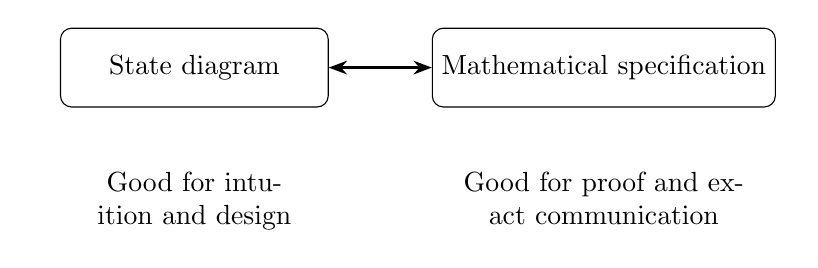
\begin{tikzpicture}[node distance=5.2cm]

\node[draw,rounded corners,minimum width=3.4cm,minimum height=1cm] (g)
{State diagram};

\node[draw,rounded corners,minimum width=4.2cm,minimum height=1cm,right of=g] (m)
{Mathematical specification};

\draw[<->,>=Stealth,thick] (g) -- (m);

\node[below=0.7cm of g,text width=4cm,align=center]
{Good for intuition and design};

\node[below=0.7cm of m,text width=4.5cm,align=center]
{Good for proof and exact communication};

\end{tikzpicture}
\end{center}

\vspace{1em}

A transition table is simply one convenient way to define the transition function.

\end{frame}

%================================================
\begin{frame}{A DFA Has Five Ingredients}

To describe a deterministic finite automaton, we need:

%\pause

\begin{enumerate}
\item a finite set of states,
%\pause
\item an input alphabet,
%\pause
\item a rule for moving between states,
%\pause
\item a start state,
%\pause
\item a set of accepting states.
\end{enumerate}

%\pause

So we write
\[
\dfa.
\]

\end{frame}

%================================================
\begin{frame}{Definition: Deterministic Finite Automaton}

A \textbf{deterministic finite automaton}, or DFA, is a 5-tuple
\[
M=(Q,\Sigma,\delta,q_0,F),
\]
where

\begin{itemize}
\item $Q$ is a finite set of states,
\item $\Sigma$ is a finite input alphabet,
\item $\delta:Q\times\Sigma\rightarrow Q$ is the transition function,
\item $q_0\in Q$ is the start state,
\item $F\subseteq Q$ is the set of accepting states.
\end{itemize}

\end{frame}

%================================================
\begin{frame}{The Running Example: Even Number of 1's}

Language we want to recognize:
\[
\lang{EVEN}_1=\{w\in\{0,1\}^*: w\text{ contains an even number of }1\text{'s}\}.
\]

\[
\text{Members: }\eps,0,11,1010
\qquad
\text{Non-members: }1,10,111.
\]

%\pause

What information must the machine remember?

%\pause

Only whether the number of $1$'s seen so far is even or odd.

\[
q_E: \text{even number of }1\text{'s seen},
\qquad
q_O: \text{odd number of }1\text{'s seen}.
\]

\end{frame}

%================================================
\begin{frame}{The Same Machine as a Diagram}

\begin{center}
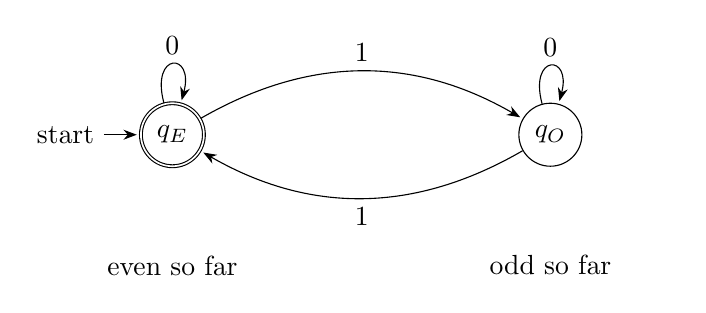
\begin{tikzpicture}[->,>=Stealth,shorten >=1pt,node distance=4.8cm]

\node[dfastate,initial,accepting] (e) {$q_E$};
\node[dfastate,right of=e] (o) {$q_O$};

\path
(e) edge[loop above] node {$0$} ()
(e) edge[bend left] node[above] {$1$} (o)
(o) edge[loop above] node {$0$} ()
(o) edge[bend left] node[below] {$1$} (e);

\node[below=1.0cm of e,text width=3cm,align=center] {even so far};
\node[below=1.0cm of o,text width=3cm,align=center] {odd so far};

\end{tikzpicture}
\end{center}

\vspace{0.5em}

States are not merely circles; they encode the information remembered by the machine.

\end{frame}

%================================================
\begin{frame}{The Same Machine as Mathematics}

\[
Q=\{q_E,q_O\},
\qquad
\Sigma=\{0,1\},
\qquad
q_0=q_E,
\qquad
F=\{q_E\}.
\]

%\pause

The transition function $\delta$ is defined by
\[
\begin{array}{c|cc}
\delta & 0 & 1\\
\hline
q_E & q_E & q_O\\
q_O & q_O & q_E
\end{array}
\]

%\pause

This table is not a third representation; it is simply a compact definition of $\delta$.

\end{frame}

%================================================
\begin{frame}{Why Is It Called Deterministic?}

For every pair
\[
(q,a)\in Q\times\Sigma,
\]
there is exactly one next state
\[
\delta(q,a)\in Q.
\]

\vspace{1em}

%\pause

No guessing.

No ambiguity.

No missing transition.

Exactly one next state.

\end{frame}

%================================================
\begin{frame}[standout]
A DFA is finite memory plus a deterministic update rule.
\end{frame}

%================================================
\section{3B. Acceptance, Rejection, and Languages}

%================================================
\begin{frame}{Formal Acceptance}

Let
\[
M=(Q,\Sigma,\delta,q_0,F)
\]
be a DFA, and let
\[
w=w_1w_2\cdots w_n
\]
be an input string over $\Sigma$.

%\pause

The machine accepts $w$ if there is a sequence of states
\[
r_0,r_1,\ldots,r_n
\]
such that

\begin{enumerate}
\item $r_0=q_0$,
\item $\delta(r_i,w_{i+1})=r_{i+1}$ for $0\le i\le n-1$,
\item $r_n\in F$.
\end{enumerate}

\end{frame}

%================================================
\begin{frame}{Language of a DFA}

\begin{block}{}
Let $M$ be a DFA. The \textbf{language of $M$} is
\[
L(M)=\{w\in\Sigma^*: M\text{ accepts }w\}.
\]

A DFA $M$ \textbf{accepts} or \textbf{recognizes} a language $L$ when
\[
L(M)=L.
\]
\end{block}

%\pause

So for the intended language $L$:
\[
w\in L \Rightarrow M\text{ accepts }w,
\qquad
w\notin L \Rightarrow M\text{ rejects }w.
\]

\end{frame}

%================================================
\begin{frame}{What About the Empty String?}

The empty string is
\[
\eps.
\]

It has length zero.

%\pause

If the input is $\eps$, the DFA reads no symbols.

%\pause

So it remains in the start state $q_0$.

%\pause

Therefore:

\begin{center}
A DFA accepts $\eps$ exactly when $q_0\in F$.
\end{center}

\end{frame}

%================================================
\begin{frame}{Three Similar-Looking Objects}

These are different:

\vspace{0.5em}

\begin{center}
\begin{tabular}{lll}
\toprule
\textbf{Notation} & \textbf{Meaning} & \textbf{Size}\\
\midrule
$\eps$ & the empty string & length $0$\\
$\emptyset$ & the empty language & $0$ strings\\
$\{\eps\}$ & language containing only the empty string & $1$ string\\
\bottomrule
\end{tabular}
\end{center}

%\pause

\vspace{1em}

Common mistake:
\[
\emptyset \ne \{\eps\}.
\]

\end{frame}

%================================================
\begin{frame}{Dead States}

A dead state represents a situation from which success is impossible.

%\pause

Once the machine enters a dead state, it stays there forever.

\begin{center}
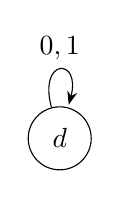
\begin{tikzpicture}[->,>=Stealth,shorten >=1pt,node distance=3cm]
\node[dfastate] (d) {$d$};
\path (d) edge[loop above] node {$0,1$} ();
\end{tikzpicture}
\end{center}

%\pause

Dead states ensure the automaton mathematically remains deterministic and complete.

\end{frame}

%================================================
\section{3C. Worked Examples: Designing States}

%================================================
\begin{frame}{How to Design a DFA}

A good design strategy:

\begin{enumerate}
\item Decide what information must be remembered.
\item Make one state for each possible memory situation.
\item Define how each input symbol updates that information.
\item Mark the accepting states.
\end{enumerate}

%\pause

The hardest step is almost always the first one.

\begin{center}
What finite information is enough?
\end{center}

\end{frame}

%================================================
\begin{frame}{Example 1: Strings Containing 001}

Language:
\[
L=\{w\in\{0,1\}^*: w\text{ contains }001\text{ as a substring}\}.
\]

\[
\text{Members: }001,1001,0010
\qquad
\text{Non-members: }\eps,00,0101.
\]

%\pause

What should the states remember?

%\pause

The longest suffix of the input so far that is also a prefix of $001$.

\begin{itemize}
\item nothing useful yet,
\item just saw $0$,
\item just saw $00$,
\item have seen $001$.
\end{itemize}

\end{frame}

%================================================
\begin{frame}{DFA for Strings Containing 001}

\begin{center}
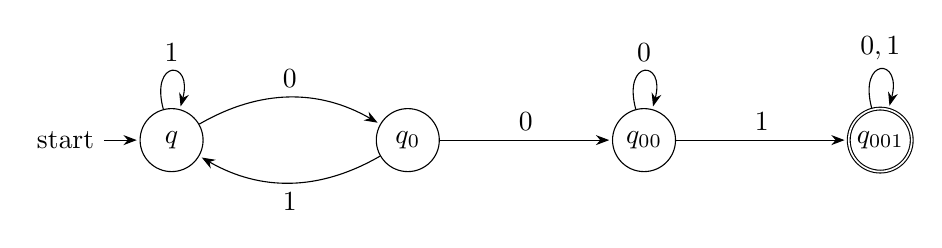
\begin{tikzpicture}[->,>=Stealth,shorten >=1pt,node distance=3.0cm]

\node[dfastate,initial] (q0) {$q$};
\node[dfastate,right of=q0] (q1) {$q_0$};
\node[dfastate,right of=q1] (q2) {$q_{00}$};
\node[dfastate,accepting,right of=q2] (q3) {$q_{001}$};

\path
(q0) edge[loop above] node {$1$} ()
(q0) edge[bend left] node[above] {$0$} (q1)
(q1) edge[bend left] node[below] {$1$} (q0)
(q1) edge node[above] {$0$} (q2)
(q2) edge[loop above] node {$0$} ()
(q2) edge node[above] {$1$} (q3)
(q3) edge[loop above] node {$0,1$} ();

\end{tikzpicture}
\end{center}

\vspace{0.5em}

A doubly circled state means an accepting state. 

\end{frame}

%================================================
\begin{frame}{Example 2: Binary Numbers Divisible by 3}

Language:
\[
L=\{w\in\{0,1\}^+: w\text{ is the binary representation of a number divisible by }3\}.
\]

\[
\text{Members: }0,11,110,1001
\qquad
\text{Non-members: }\eps,1,10,100.
\]

%\pause

At first this looks arithmetic, not automata. But we only need to remember the remainder modulo $3$.

\[
q_s: \text{no bit read yet},
\qquad
q_0: \text{rem }0,
\qquad
q_1: \text{rem }1,
\qquad
q_2: \text{rem }2.
\]

\begin{block}{Special Note: $*$ vs $+$}
$\Sigma^*$ means zero or more symbols, so $\eps\in\Sigma^*$.
$\Sigma^+$ means one or more symbols, so $\eps\notin\Sigma^+$.
\end{block}

\end{frame}

%================================================
\begin{frame}{Updating Remainders}

If the current value has remainder $r$ modulo $3$, and we append bit $b$, the new value is
\[
2r+b \pmod 3.
\]

Why? Appending a bit to the right doubles the old binary number and adds the new bit.

%\pause

So the transition rule is
\[
r\mapsto 2r+b \pmod 3.
\]

\end{frame}

%================================================
\begin{frame}{DFA for Divisibility by 3}

\begin{center}
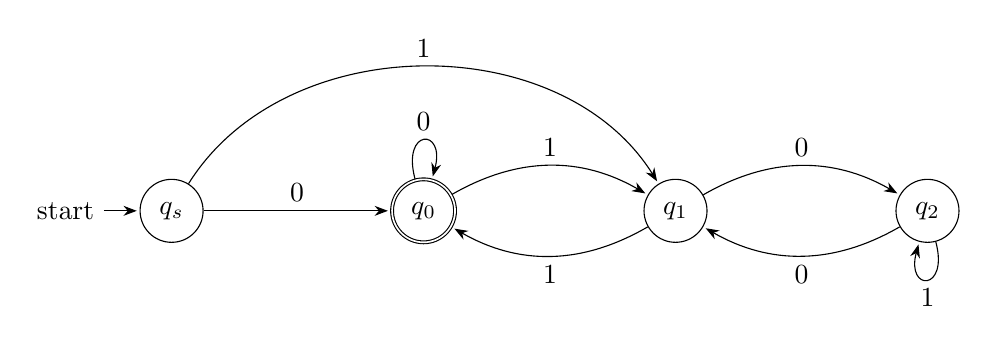
\begin{tikzpicture}[->,>=Stealth,shorten >=1pt,node distance=3.2cm]

\node[dfastate,initial] (qs) {$q_s$};
\node[dfastate,accepting,right of=qs] (q0) {$q_0$};
\node[dfastate,right of=q0] (q1) {$q_1$};
\node[dfastate,right of=q1] (q2) {$q_2$};

\path
(qs) edge node[above] {$0$} (q0)
(qs) edge[bend left=58] node[above] {$1$} (q1)
(q0) edge[loop above] node {$0$} ()
(q0) edge[bend left] node[above] {$1$} (q1)
(q1) edge[bend left] node[below] {$1$} (q0)
(q1) edge[bend left] node[above] {$0$} (q2)
(q2) edge[bend left] node[below] {$0$} (q1)
(q2) edge[loop below] node {$1$} ();

\end{tikzpicture}
\end{center}

Accept when at least one bit has been read and the remainder is $0$.

\end{frame}

%================================================
\begin{frame}{Example 3: Valid Football Scores}

Language over $\Sigma=\{0,d,-\}$, where $d$ means any nonzero digit:
\[
L=\{x-y: x,y\text{ are nonnegative integers with no leading zeros}\}.
\]

\[
\text{Members: }\text{\texttt{0-0}},\ \text{\texttt{d-0}},\ \text{\texttt{d0-dd}}
\qquad
\text{Non-members: }\eps,\ \text{\texttt{00-d}},\ \text{\texttt{d-}},\ \text{\texttt{d--0}}.
\]

%\pause

What must the state remember?
\begin{itemize}
\item Are we reading the first score or the second score?
\item Did the current score start with $0$ or with a nonzero digit?
\item Have we already used the single hyphen?
\end{itemize}

\end{frame}

%================================================
\begin{frame}{DFA for Valid Football Scores}

\begin{center}
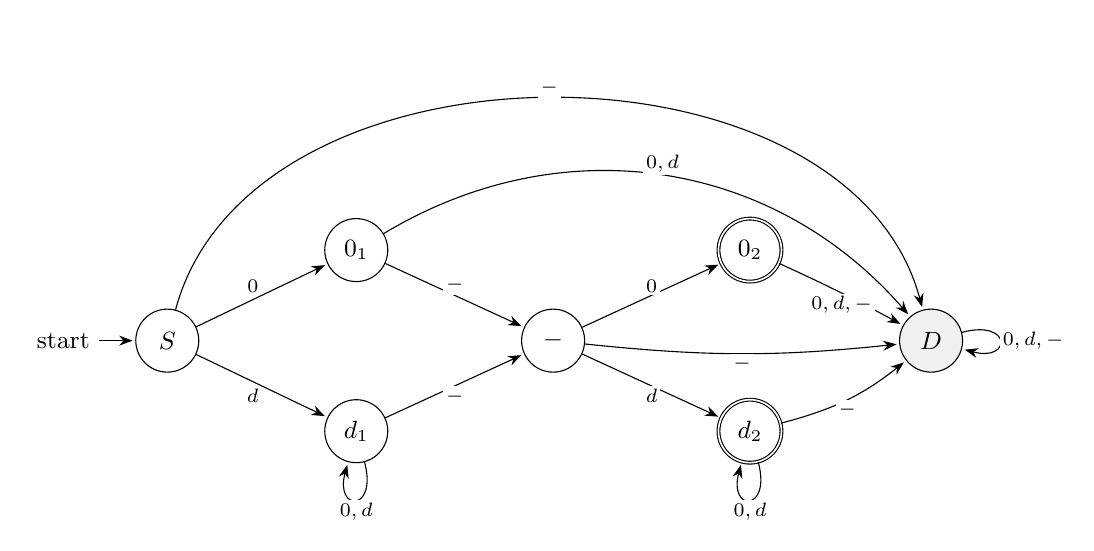
\begin{tikzpicture}[
  ->,>=Stealth,shorten >=1pt,
  state/.style={circle,draw,minimum size=8mm,inner sep=1pt},
  accept/.style={state,double},
  dead/.style={state,fill=black!6},
  every node/.style={font=\small},
  lab/.style={font=\scriptsize,fill=white,inner sep=1pt}
]

\node[state,initial] (S) at (0,0) {$S$};

\node[state] (Z1) at (2.4,1.15) {$0_1$};
\node[state] (N1) at (2.4,-1.15) {$d_1$};

\node[state] (H) at (4.9,0) {$-$};

\node[accept] (Z2) at (7.4,1.15) {$0_2$};
\node[accept] (N2) at (7.4,-1.15) {$d_2$};

\node[dead] (D) at (9.7,0) {$D$};

\path
(S) edge node[lab,above left] {$0$} (Z1)
(S) edge node[lab,below left] {$d$} (N1)
(S) edge[bend left=75] node[lab,above] {$-$} (D)

(Z1) edge node[lab,above] {$-$} (H)
(Z1) edge[bend left=40] node[lab,above] {$0,d$} (D)

(N1) edge[loop below] node[lab] {$0,d$} ()
(N1) edge node[lab,below] {$-$} (H)

(H) edge node[lab,above] {$0$} (Z2)
(H) edge node[lab,below] {$d$} (N2)
(H) edge[bend right=6] node[lab,below] {$-$} (D)

(Z2) edge[bend left=2] node[lab,below] {$0,d,-$} (D)

(N2) edge[loop below] node[lab] {$0,d$} ()
(N2) edge[bend right=12] node[lab,below] {$-$} (D)

(D) edge[loop right] node[lab] {$0,d,-$} ();

\end{tikzpicture}
\end{center}

% \vspace{0.3em}
% \small A single $0$ is allowed, but $00$ is not a valid score component.

\end{frame}
%================================================
\section{3D. Advanced Examples: Pushing the Limits}

%================================================
\begin{frame}{Advanced Example 1: The Product Construction Concept}

Language over $\Sigma = \{0, 1\}$:
\[
L=\{w : w\text{ has an even number of } 0\text{'s \textbf{AND} its length is a multiple of } 3\}.
\]

\[
\text{Members: }\eps,111,001
\qquad
\text{Non-members: }0,11,011.
\]

%\pause

We must track \textbf{two} independent pieces of information simultaneously:
\begin{enumerate}
\item Parity of $0$'s (Even or Odd) $\to$ 2 possibilities
\item Length modulo 3 (0, 1, or 2) $\to$ 3 possibilities
\end{enumerate}

%\pause

Total states required: $2 \times 3 = 6$. A state is a pair $(p, l)$.

\end{frame}

%================================================
\begin{frame}{DFA for Multiple Conditions}

\begin{center}
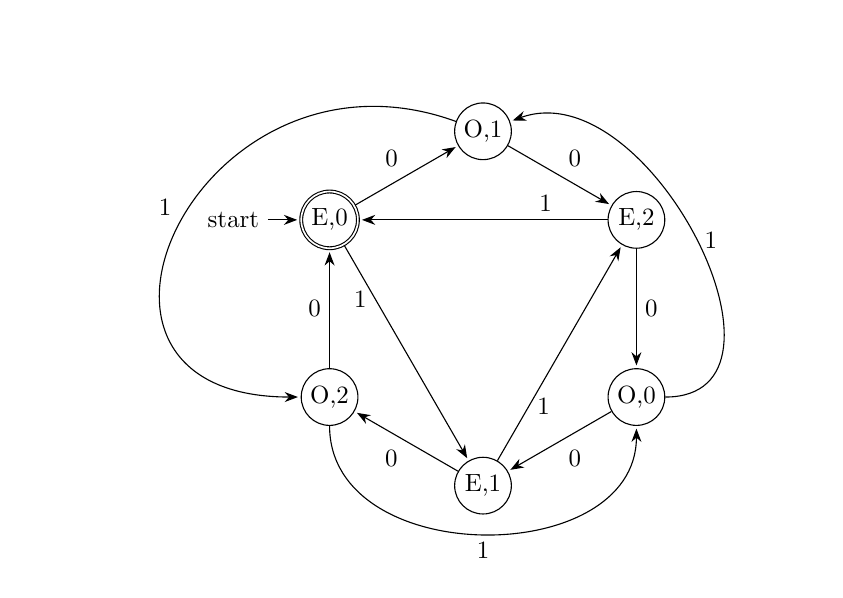
\begin{tikzpicture}[->,>=Stealth,shorten >=1pt,scale=0.9, transform shape]

% Arrange states in a hexagon based on the 0-transition cycle
\node[dfastate,initial,accepting] (e0) at (150:2.5cm) {E,0};
\node[dfastate] (o1) at (90:2.5cm) {O,1};
\node[dfastate] (e2) at (30:2.5cm) {E,2};
\node[dfastate] (o0) at (-30:2.5cm) {O,0};
\node[dfastate] (e1) at (-90:2.5cm) {E,1};
\node[dfastate] (o2) at (-150:2.5cm) {O,2};

% 0-transitions (outer perimeter of the hexagon)
\path
(e0) edge node[above left] {$0$} (o1)
(o1) edge node[above right] {$0$} (e2)
(e2) edge node[right] {$0$} (o0)
(o0) edge node[below right] {$0$} (e1)
(e1) edge node[below left] {$0$} (o2)
(o2) edge node[left] {$0$} (e0);

% 1-transitions for E states (straight chords INSIDE the hexagon)
\path
(e0) edge node[left,near start] {$1$} (e1)
(e1) edge node[right,near start] {$1$} (e2)
(e2) edge node[above,near start] {$1$} (e0);

% 1-transitions for O states (curved edges OUTSIDE the hexagon)
% \path
% (o0) edge[bend right=50] node[right] {$1$} (o1)
% (o1) edge[bend right=50] node[above left] {$1$} (o2)
% (o2) edge[bend right=50] node[below] {$1$} (o0);
\path
(o0) edge[out=0,in=20,looseness=1.2] node[right] {$1$} (o1)
(o1) edge[out=160,in=-180,looseness=2.2] node[above left] {$1$} (o2)
(o2) edge[out=-90,in=-90,looseness=1.2] node[below] {$1$} (o0);

\end{tikzpicture}
\end{center}


\end{frame}
%================================================
\begin{frame}{Advanced Example 2: The $k$-th Symbol from the End}

Language:
\[
L=\{w\in\{0,1\}^*: \text{the } 2\text{nd symbol from the right is a } 1\}.
\]

\[
\text{Members: }10,011,110,0011
\qquad
\text{Non-members: }\eps,0,1,100.
\]

%\pause
\vspace{1em}

What must the state remember?
%\pause
It must act like a sliding window, remembering the \textbf{last 2 symbols} seen.
States: $q_{00}, q_{01}, q_{10}, q_{11}$.

\vspace{1em}
If we are in $q_{01}$ (last two symbols were $0,1$) and we read a $0$, our new ``last two symbols'' are $1,0$. Thus, $q_{01} \xrightarrow{0} q_{10}$.

\end{frame}

%================================================
\begin{frame}{DFA for the 2nd Symbol from the Right}

\begin{center}
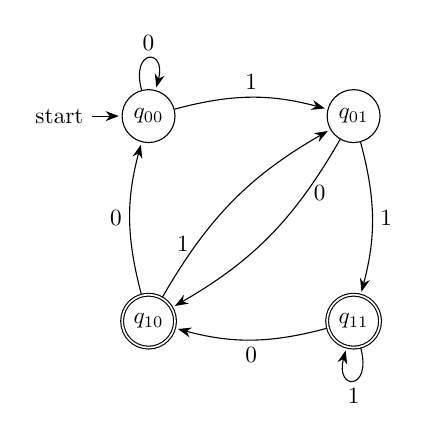
\begin{tikzpicture}[->,>=Stealth,shorten >=1pt,node distance=3.1cm,scale=0.84,transform shape]

\node[dfastate,initial] (q00) {$q_{00}$};
\node[dfastate,right of=q00] (q01) {$q_{01}$};
\node[dfastate,accepting,below of=q00] (q10) {$q_{10}$};
\node[dfastate,accepting,below of=q01] (q11) {$q_{11}$};

\path
(q00) edge[loop above] node {$0$} ()
(q00) edge[bend left=15] node[above] {$1$} (q01)
(q01) edge[bend left=15] node[near start,right] {$0$} (q10)
(q01) edge[bend left=15] node[right] {$1$} (q11)
(q10) edge[bend left=15] node[left] {$0$} (q00)
(q10) edge[bend left=15] node[near start,left] {$1$} (q01)
(q11) edge[bend left=15] node[below] {$0$} (q10)
(q11) edge[loop below] node {$1$} ();

\end{tikzpicture}
\end{center}

\vspace{0.5em}
\scriptsize{\textit{Initial state $q_{00}$ pretends we have seen leading zeros.}}

\end{frame}

%================================================
\begin{frame}{Advanced Example 3: Pattern Interference}

Language over $\Sigma = \{a, b\}$:
\[
L=\{w : w\text{ contains } ab \text{ as a substring, but does \textbf{not} contain } ba\}.
\]

\[
\text{Members: }ab,aab,abb,aaabbb
\qquad
\text{Non-members: }\eps,a,b,aba,ba.
\]

%\pause

Think about the structure of valid strings:
\begin{itemize}
\item They must eventually contain $ab$.
\item Once a $b$ occurs, no $a$ can \textit{ever} follow it (otherwise we get $ba$).
\item Therefore, valid strings look exactly like $a^+ b^+$.
\end{itemize}

%\pause
States needed: start, reading $a$'s, started with $b$'s, seen $ab$, and dead after $ba$.

\end{frame}

%================================================
\begin{frame}{DFA for Pattern Interference}

\begin{center}
\begin{tikzpicture}[->,>=Stealth,shorten >=1pt,node distance=2.5cm]

\node[smallstate,initial] (S) {S};
\node[smallstate,right of=S, yshift=1.5cm] (A) {A};
\node[smallstate,right of=S, yshift=-1.5cm] (B) {B};
\node[smallstate,accepting,right of=A, xshift=1.5cm] (AB) {AB};
\node[smallstate,right of=B, xshift=1.5cm] (D) {Dead};

\path
(S) edge node[above left] {$a$} (A)
(S) edge node[below left] {$b$} (B)
(A) edge[loop above] node {$a$} ()
(A) edge node[above] {$b$} (AB)
(B) edge[loop below] node {$b$} ()
(B) edge node[below] {$a$} (D)
(AB) edge[loop right] node {$b$} ()
(AB) edge node[right] {$a$} (D)
(D) edge[loop right] node {$a,b$} ();

\end{tikzpicture}
\end{center}

\vspace{0.5em}
Notice how starting with $b$ means the string can never contain $ab$ without first producing $ba$.

\end{frame}

%================================================
\begin{frame}{Advanced Example 4: No Symbol Repeated}

Language over $\Sigma=\{a,b,c\}$:
\[
L=\{w\in\{a,b,c\}^*: \text{no symbol appears more than once in }w\}.
\]

\[
\text{Members: }\eps,a,ba,cab,bca
\qquad
\text{Non-members: }aa,aba,cabc,bb.
\]

%\pause

What must the state remember?

\begin{center}
The set of symbols seen so far.
\end{center}

\[
\emptyset,a,b,c,ab,bc,ca,abc
\]
plus one dead state $D$ for a repeated symbol.

\end{frame}

%================================================
\begin{frame}{DFA for No Symbol Repeated}

\small
State $x$ means the symbols in $x$ are already encountered.
All states except $D$ are accepting.

\vspace{0.5em}

\begin{center}
\begin{tabular}{c|ccc}
\toprule
\textbf{State} & \textbf{on $a$} & \textbf{on $b$} & \textbf{on $c$}\\
\midrule
$\emptyset$ & $a$ & $b$ & $c$\\
$a$ & $D$ & ${ab}$ & ${ac}$\\
$b$ & ${ab}$ & $D$ & ${bc}$\\
$c$ & ${ac}$ & ${bc}$ & $D$\\
${ab}$ & $D$ & $D$ & ${abc}$\\
${ac}$ & $D$ & ${abc}$ & $D$\\
${bc}$ & ${abc}$ & $D$ & $D$\\
${abc}$ & $D$ & $D$ & $D$\\
$D$ & $D$ & $D$ & $D$\\
\bottomrule
\end{tabular}
\end{center}

\end{frame}

%================================================
\begin{frame}{Advanced Example 5: Lexical Analysis (C-Style Comments)}

Language over $\Sigma = \{/, *, x\}$ (where $x$ is any other char):
\[
L=\{w : w\text{ is exactly one valid block comment starting with /* and ending with */} \}.
\]

\[
\text{Members: }\text{\texttt{/**/}},\text{\texttt{/*x*/}},\text{\texttt{/*/x**/}}
\qquad
\text{Non-members: }\text{\texttt{/*}},\text{\texttt{/x*/}},\text{\texttt{/*x*/x}},\text{\texttt{/*x*/*/}}.
\]

\begin{block}{Valid block comment}
A valid block comment starts with \texttt{/*}, ends at the first later \texttt{*/}, and has no extra symbols after that closing delimiter.
\end{block}

\end{frame}

%================================================
\begin{frame}{DFA for C-Style Comments}

\begin{center}
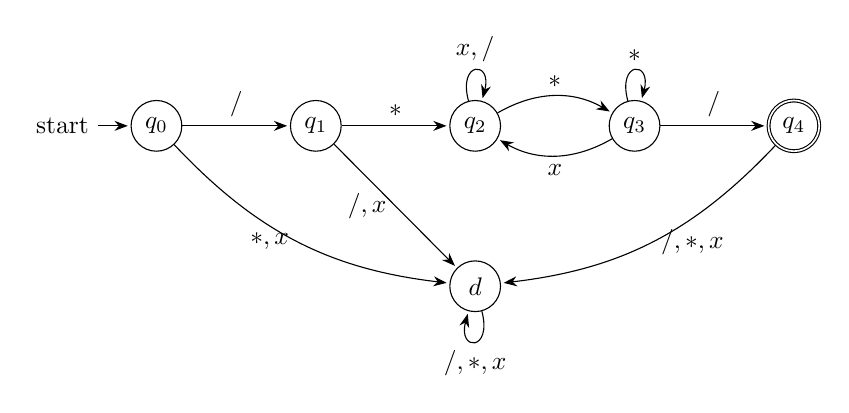
\begin{tikzpicture}[->,>=Stealth,shorten >=1pt,node distance=2.2cm,scale=0.92,transform shape]

\node[smallstate,initial] (q0) {$q_0$};
\node[smallstate,right of=q0] (q1) {$q_1$};
\node[smallstate,right of=q1] (q2) {$q_2$};
\node[smallstate,right of=q2] (q3) {$q_3$};
\node[smallstate,accepting,right of=q3] (q4) {$q_4$};
\node[smallstate,below=1.5cm of q2] (d) {$d$};

\path
(q0) edge node[above] {$/$} (q1)
(q1) edge node[above] {$*$} (q2)
(q2) edge[bend left] node[above] {$*$} (q3)
(q3) edge node[above] {$/$} (q4)
(q3) edge[bend left] node[below] {$x$} (q2)
(q3) edge[loop above] node {$*$} ()
(q2) edge[loop above] node {$x,/$} ()

(q0) edge[bend right=20] node[left] {$*,x$} (d)
(q1) edge node[left] {$/,x$} (d)
(q4) edge[bend left=20] node[right] {$/,*,x$} (d)
(d) edge[loop below] node {$/,*,x$} ();

\end{tikzpicture}
\end{center}

\vspace{0.3em}
This finite memory tracking is exactly how compilers strip comments from source code!

\end{frame}

%================================================
\begin{frame}{What You Should Be Able to Do Now}

Given a DFA, you should be able to:

\begin{itemize}
\item identify $Q,\Sigma,\delta,q_0,F$,
\item explain what each state remembers,
\item trace an input string and decide if it is accepted,
\item describe the language recognized by the DFA.
\end{itemize}

%\pause

Given a language description, you should begin by asking:

\begin{center}
\textbf{What finite information is enough?}
\end{center}

\end{frame}

%================================================
\begin{frame}[standout]
A DFA is not merely a diagram.

It is a mathematical object that computes using finite memory.
\end{frame}

%================================================
\end{document}
